%%%%%%%%%%%%%%%%%%%%%%%%%%%%%%%%%%%%%%%%%%%%%%%%%%%%%%%%%%%%%%%%
%%%%%%%%%%%%%%%%%%%%%%%%%%%%%%%%%%%%%%%%%%%%%%%%%%%%%%%%%%%%%%%%
%%%%
%%%% This text file is part of the source of slides for
%%%% `Introduction to High-Performance Scientific Computing'
%%%% by Victor Eijkhout, copyright 2012
%%%%
%%%%%%%%%%%%%%%%%%%%%%%%%%%%%%%%%%%%%%%%%%%%%%%%%%%%%%%%%%%%%%%%
%%%%%%%%%%%%%%%%%%%%%%%%%%%%%%%%%%%%%%%%%%%%%%%%%%%%%%%%%%%%%%%%

\documentclass[headnav]{beamer}

\newenvironment{beamdisplayeq}%
 {\begin{equation}\small}{\end{equation}}

\usepackage{beamerthemeTACC}
\parskip=.5\baselineskip plus .5\baselineskip
\event{PCSE 2013}

\usepackage{amsmath,arydshln,graphicx,comment,multicol,undertilde}
\usepackage{hyperref}

\newcommand\inv{^{-1}}

\usepackage[algo2e]{algorithm2e}
\newenvironment{displayalgorithm}
 {\begin{algorithm2e}[H]}{\end{algorithm2e}}
\newenvironment{displayprocedure}[2]
 {\begin{procedure}[H]\caption{#1(#2)}}
 {\end{procedure}}
\def\sublocal{_{\mathrm\scriptstyle local}}

\begin{document}
\title{Scalability of Collective Operations}
\author{Victor Eijkhout}
\date{}
\frame{\titlepage}


\frame{\tableofcontents}

\sectionframe{Cost analysis}
\frame{\frametitle{Concepts}
  \begin{itemize}
  \item $\alpha$: message latency
  \item $\beta$: transfer time per byte
  \item $\gamma$: time for floating point operation
  \end{itemize}
Recall definitions of weak/strong scalability
}

\sectionframe{Dense matrix-vector product}

\frame{\frametitle{Parallel matrix-vector product; dense}
  \begin{itemize}
  \item Assume a division by block rows
  \item Every processor $p$ has a set of row indices $I_p$
  \end{itemize}
  Mvp on processor $p$: \[ \forall_i\colon y_i=\sum_j a_{ij}x_j \]
  \[ \forall_i\colon y_i=\sum_q\sum_{j\in I_q} a_{ij}x_j \]
}

\frame{\frametitle{}
Local and remote parts:

  \[ \forall_i\colon y_i=\sum_{j\in
    I_p}a_{ij}x_j+\sum_{q\not=p}\sum_{j\in I_q} a_{ij}x_j 
  \]
  Each processor needs to collect the whole vector: Allgather

  Combine:
  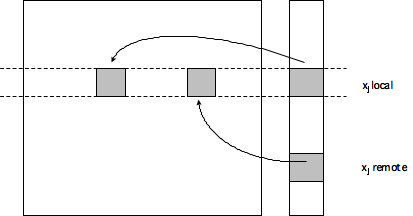
\includegraphics[scale=.6]{distmvp}
}

\frame{\frametitle{Cost computation 1.}
Algorithm:
\begin{center}
\begin{tabular}{| p{2in} |  p{2in} |}\hline
Step & Cost (lower bound) \\ \hline
Allgather $ x_i $ so that $ x $ is available on all nodes & \\
Locally compute $ y_i = A_i x $ &
$ \approx 2 \frac{n^2}{P} \gamma $ \\ \hline
\end{tabular}
\end{center}

}

\frame{\frametitle{Allgather}
Assume that data arrives over a binary tree:
\begin{itemize}
\item latency $\alpha\log_2 P$
\item transmission time, receiving $n/P$ elements from $P-1$ processors
\end{itemize}
}

\frame{\frametitle{}
Algorithm with cost:
\begin{center}
\begin{tabular}{| p{2in} |  p{2in} |}\hline
Step & Cost (lower bound) \\ \hline
Allgather $ x_i $ so that $ x $ is available on all nodes & 
$ \lceil \log_2(P)\rceil \alpha + \frac{P-1}{P} n \beta \approx
\log_2(P) \alpha + n \beta $ \\
Locally compute $ y_i = A_i x $ &
$ \approx 2 \frac{n^2}{P} \gamma $ \\ \hline
\end{tabular}
\end{center}

}

\frame{\frametitle{Parallel efficiency}
\[
E_p^{\mbox{1D-row}}(n) = 
\frac{S_p^{\mbox{1D-row}}(n)}{p}
= 
\frac{1}
{ 1 + \frac{p \log_2(p)}{2 n^2} \frac{\alpha}{\gamma} 
+ \frac{p}{2 n} \frac{\beta}{\gamma} }.
\]
Strong scaling, weak scaling?
}

\frame{\frametitle{Two-dimensional partitioning}
{\tiny
\[
\begin{array}{| c | c | c | c |} \hline
% 0,0
\begin{array}{c c c c}
x_0\\
a_{00} & a_{01} &a_{02} & y_0\\
a_{10} & a_{11} &a_{12} & \\
a_{20} & a_{21} &a_{22} & \\
a_{30} & a_{31} &a_{32} & \\
\end{array}
&
% 0,1
\begin{array}{c c c c}
x_3\\
a_{03} & a_{04} &a_{05} & \\
a_{13} & a_{14} &a_{15} & y_1\\
a_{23} & a_{24} &a_{25} & \\
a_{33} & a_{34} &a_{35} & \\
\end{array}
&
% 0,2
\begin{array}{c c c c}
x_6\\
a_{06} & a_{07} &a_{08} & \\
a_{16} & a_{17} &a_{18} & \\
a_{26} & a_{27} &a_{28} & y_2 \\
a_{37} & a_{37} &a_{38} & \\
\end{array}
&
% 0,3
\begin{array}{c c c c}
x_9\\
a_{09} & a_{0,10} & a_{0,11} & \\
a_{19} & a_{1,10} & a_{1,11} & \\
a_{29} & a_{2,10} & a_{2,11} & \\
a_{39} & a_{3,10} & a_{3,11} & y_3 \\
\end{array}
\\ \hline
% 1,0
\begin{array}{c c c c}
& x_1\\
a_{40} & a_{41} &a_{42} & y_4\\
a_{50} & a_{51} &a_{52} & \\
a_{60} & a_{61} &a_{62} & \\
a_{70} & a_{71} &a_{72} & \\
\end{array}
&
% 1,1
\begin{array}{c c c c}
& x_4\\
a_{43} & a_{44} &a_{45} & \\
a_{53} & a_{54} &a_{55} & y_5\\
a_{63} & a_{64} &a_{65} & \\
a_{73} & a_{74} &a_{75} & \\
\end{array}
&
% 1,2
\begin{array}{c c c c}
& x_7\\
a_{46} & a_{47} &a_{48} & \\
a_{56} & a_{57} &a_{58} & \\
a_{66} & a_{67} &a_{68} & y_6 \\
a_{77} & a_{77} &a_{78} & \\
\end{array}
&
% 1,3
\begin{array}{c c c c}
& x_{10}\\
a_{49} & a_{4,10} & a_{4,11} & \\
a_{59} & a_{5,10} & a_{5,11} & \\
a_{69} & a_{6,10} & a_{6,11} & \\
a_{79} & a_{7,10} & a_{7,11} & y_7 \\
\end{array}
\\ \hline
% 0,0
\begin{array}{c c c c}
&&x_2\\
a_{80} &  a_{81} &  a_{82} & y_8\\
a_{90} &  a_{91}   &a_{92} & \\
a_{10,0} &a_{10,1} &a_{10,2} & \\
a_{11,0} &a_{11,1} &a_{11,2} & \\
\end{array}
&
% 0,1
\begin{array}{c c c c}
&&x_5\\
a_{83} &   a_{84} &  a_{85} & \\
a_{93} &   a_{94} &  a_{95} & y_9\\
a_{10,3} & a_{10,4} &a_{10,5} & \\
a_{11,3} & a_{11,4} &a_{11,5} & \\
\end{array}
&
% 0,2
\begin{array}{c c c c}
&&x_8\\
a_{86} &   a_{87} &  a_{88} & \\
a_{96} &   a_{97} &  a_{98} & \\
a_{10,6} & a_{10,7} &a_{10,8} & y_{10} \\
a_{11,7} & a_{11,7} &a_{11,8} & \\
\end{array}
&
% 0,3
\begin{array}{c c c c}
&&x_{11}\\
a_{89} &   a_{8,10} &  a_{8,11} & \\
a_{99} &   a_{9,10} &  a_{9,11} & \\
a_{10,9} & a_{10,10} & a_{10,11} & \\
a_{11,9} & a_{11,10} & a_{11,11} & y_{11} \\
\end{array}
\\ \hline
\end{array}
\]
}
}

\frame{\frametitle{Algorithm}
\begin{itemize}
\item Collecting $x_j$ on each processor $p_{ij}$ by an
  \emph{allgather} inside the processor columns.
\item Each processor $p_{ij}$ then computes $y_{ij} = A_{ij}x_j$.
\item Gathering together the pieces $y_{ij}$ in each processor row to
  form~$y_i$, distribute this over the processor row: combine to form
  a \emph{reduce-scatter}.
\item Setup for the next $A$ or $A^t$ product
\end{itemize}
}

\frame{\frametitle{Analysis 1.}
\begin{tabular}{| p{2in} |  p{2in} |}\hline
Step & Cost (lower bound) \\ \hline
Allgather $ x_i $'s  within columns & 
$ \lceil \log_2(r)\rceil \alpha + \frac{r-1}{p} n \beta \approx
\log_2(r) \alpha + \frac{n}{c} \beta $ \\
Perform local matrix-vector multiply &
$ \approx 2 \frac{n^2}{p} \gamma $ \\ 
Reduce-scatter $ y_i $'s  within rows & \\ \hline
\end{tabular}
}

\frame{\frametitle{Reduce-scatter}
{\footnotesize
\[
\begin{array}{|c|cccc|}
\hline
  &t=1&t=2&t=3\\ \hline
p_0&x_0^{(0)},x_1^{(0)},x_2^{(0)}\downarrow,x_3^{(0)}\downarrow
   &x_0^{(0:2:2)},x_1^{(0:2:2)}\downarrow
    \hphantom{x_0^{(0:2:2)},x_1^{(0:2:2)}\downarrow}
   &x_0^{(0:3)}
    \hphantom{x_3^{(0:3)}x_3^{(0:3)}x_3^{(0:3)}}\\
p_1&x_0^{(1)},x_1^{(1)},x_2^{(1)}\downarrow,x_3^{(1)}\downarrow
   &x_0^{(1:3:2)}\uparrow,x_1^{(1:3:2)}
    \hphantom{x_0^{(0:2:2)},x_1^{(0:2:2)}\downarrow}
   &\hphantom{x_3^{(0:3)}} x_1^{(0:3)}
    \hphantom{x_3^{(0:3)}x_3^{(0:3)}} \\
p_2&x_0^{(2)}\uparrow,x_1^{(2)}\uparrow,x_2^{(2)},x_3^{(2)}
   &\hphantom{x_0^{(0:2:2)},x_1^{(0:2:2)}\downarrow}
    x_2^{(0:2:2)},x_3^{(0:2:2)}\downarrow
   &\hphantom{x_3^{(0:3)}x_3^{(0:3)}} x_2^{(0:3)}
    \hphantom{x_3^{(0:3)}}\\
p_3&x_0^{(3)}\uparrow,x_1^{(3)}\uparrow,x_2^{(3)},x_3^{(3)}
   &\hphantom{x_0^{(0:2:2)},x_1^{(0:2:2)}\downarrow}
    x_0^{(1:3:2)}\uparrow,x_1^{(1:3:2)}
   &\hphantom{x_3^{(0:3)}x_3^{(0:3)}x_3^{(0:3)}}
    x_3^{(0:3)}\\
\hline
\end{array}
\]
}
Time:
\[ \lceil \log_2 p\rceil\alpha +\frac{p-1}pn(\beta+\gamma). \]
}

\frame{\frametitle{}
\begin{tabular}{| p{2in} |  p{2in} |}\hline
Step & Cost (lower bound) \\ \hline
Allgather $ x_i $'s  within columns & 
$ \lceil \log_2(r)\rceil \alpha + \frac{r-1}{p} n \beta \approx
\log_2(r) \alpha + \frac{n}{c} \beta $ \\
Perform local matrix-vector multiply &
$ \approx 2 \frac{n^2}{p} \gamma $ \\ 
Reduce-scatter $ y_i $'s  within rows & 
$ \lceil \log_2(c)\rceil \alpha + \frac{c-1}{p} n \beta + \frac{c-1}{p} n \gamma \approx
\log_2(r) \alpha + \frac{n}{c} \beta + \frac{n}{c} \gamma $ \\ \hline
\end{tabular}
}

\frame{\frametitle{Efficiency}
\[
E_p^{\sqrt{p} \times \sqrt{p}}(n) = 
\frac{1}
{ 1 + \frac{p \log_2(p)}{2 n^2} \frac{\alpha}{\gamma} 
+ \frac{\sqrt{p}}{2n}\frac{
\left( 2 \beta + \gamma \right)}{\gamma}}
\]
Weak scaling:\\
for $p\rightarrow\infty$ this is $\approx 1/\log_2P$:\\
only slowly decreasing.
}

\end{document}

\frame{\frametitle{Variable reordering}
\footnotesize
\[ 
\begin{pmatrix}
  a_{11}&a_{12}&&&&\emptyset\\ a_{21}&a_{22}&a_{23}\\ 
  &a_{32}&a_{33}&a_{34}\\ \emptyset&&\ddots&\ddots&\ddots
\end{pmatrix}
\begin{pmatrix}  x_1\\ x_2\\ x_3\\ \vdots\end{pmatrix} =
\begin{pmatrix}  y_1\\ y_2\\ y_3\\ \vdots\end{pmatrix}
\]
with redblack
\[ 
\begin{pmatrix}
  a_{11}&&&&a_{12}\\ &a_{33}&&&a_{32}&a_{34}\\ &&a_{55}&&&\ddots&\ddots\\
  &&&\ddots\\
  a_{21}&a_{23}&&&a_{22}\\ &a_{43}&a_{45}&&&a_{44}\\ &&\ddots&\ddots&&&\ddots
\end{pmatrix}
\begin{pmatrix}  x_1\\ x_3\\ x_5\\ \vdots\\ x_2\\ x_4\\ \vdots\end{pmatrix} =
\begin{pmatrix}  y_1\\ y_3\\ y_5\\ \vdots\\ y_2\\ y_4\\ \vdots\end{pmatrix}
\]
Two-processor parallel Gauss-Seidel or ILU
}

\frame{\frametitle{2D redblack}
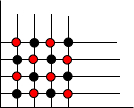
\includegraphics{graphics/redblack}

In general, colouring, colour number
}

\frame{\frametitle{Turning implicit operations into explicit}
Normalize ILU solve to $(I-L)$ and $(I-U)$

Approximate $(I-L)x = y$ by $x\approx (I+L+L^2)y$

Convergence guaranteed for diagonally dominant
}


\frame{\frametitle{}
}

\frame{\frametitle{}
}


